\documentclass{article}
\usepackage{float}
\usepackage{wrapfig}
\usepackage{graphicx}
\usepackage{listings}
\lstset{breaklines=true, breakatwhitespace=true}

\usepackage{amsmath}
\title{ECS 132 - Final Project}
\date{March 19, 2016}
\author{Vincent Yang, Corey Nettleblad, Andy Yang}

\begin{document}
  \pagenumbering{gobble} %gobble - no numbers
  \maketitle
  \newpage
  \pagenumbering{arabic} %roman - roman numbers (arabic numbers right now)
  \section*{Problem A}

  \subsection*{Part a}
    Our data provides us with a 95\% confidence interval of (3.555979, 3.621228). What is interesting to note here is that although this is a 95\% confidence interval, implying that we have a high confidence that the actual mean rating of men's ratings is between 3.555979 and 3.61228, the range of this confidence interval is relatively narrow: 0.056301. On a scale of a 1-5 rating scale, this confidence interval implies that our sample data is extremely close, and we are able to pinpoint with 95\% confidence that our population mean is within a range only 1.408\% (0.056301 / (5 - 1) of our rating scale. Perhaps raters tended to gravitate toward a specific rating more than others (between 3 and 4), which is reasonable as most ratings are not extreme toward either end of our rating spectrum.
  \subsection*{Part b}
    In part b, we were asked to perform the same task for women, instead of men. Our examination yielded a 95\% confidence interval of (3.529837, 3.64452). Because this data is closely related to the data from part a, it is only reasonable to make comparisons between them. We can determine immediately that the range of this interval is slightly larger than that for men: it is 0.114683. This interval represents a 2.8671\% of our 1-5 rating scale, approximately double that of men. From this, we have some evidence to raise the question: "Do women tend to rate more extremely than men?"
  \subsection*{Part c}
    Part c asked us to find a 95\% confidence interval for the difference between the mean rating of men and the mean rating of women. Before we even begin examining and creating models of our data, we can already predict that our confidence interval won't be very positive or very negative (will be relatively centered around 0), as in parts a and b we observed that confidence intervals of ratings of men and women individually were relatively similar.\\
    From our data, we drew a 95\% confidence interval of (-0.06134628, 0.06419663). As we predicted above, this confidence interval is relatively centered around 0. Because this confidence interval represents our confidence that our "population" (difference of ratings) mean is around 0, we can hypothesize that men and women's ratings could be the same (or around).
  \subsection*{Part d}
    This conclusion is logical as observed in the above parts, especially part c. From our 95\% confidence interval, we were already able to intuitively deduce that average ratings for men and women are very close. Using our significance test, we are able to formally accept, down to a 5 percent significance, that the averages for men and women's ratings are the same.
  \subsection*{Part e}
    \begin{figure}[H]
      \includegraphics[width=\linewidth]{histogram.png}
      \caption{Males and Females}
      \label{fig:hist1}
    \end{figure}
    As you can see, Males and Females gave generally the same average voting, but
    Females were slightly more inclined to rate between 4 and 5 while males often rated
    high 3's. 
  \subsection*{Part f}
    From this confidence interval, we can draw the conclusion that there is a 95\% chance that the actual population mean is within that range. We can draw the conclusion that there are approximately 0.41 (rough average difference) more men performing ratings than women.
  \subsection*{Part g}
    Finding a 95\% confidence interval for population proportion of users who are men is a relatively similar task as the one in part f. We were able to complete this task simply by providing the average of only male participants in the pbar average. From our results, we see that our confidence interval runs between 0.6802002 and 0.7390574 percent men. This data correlates with data that we obtained above, as there are clearly more men performing ratings in this data than women.
  \subsection*{Part h}
      \subsection*{Test the hypothesis that the coefficient for age is zero in a population regression based on age and gender}
        After building the linear model, I was able to pull the values for the coefficient of age and the standard error for that coefficient and place them in separate variables, which we used for a significance test. 
        \newline Although the results of the linear model and the significance test both suggest that 0 outside of the accepted range of 5 percent, if we loo at how small that actual values of the coefficient for age really are, we see that 0 is not necessarily too far off from the coefficient values. So, while the significance test rejects the Hypothesis, I would not necessarily say that 0 is an unacceptable coefficient.
      \subsection*{Form a confidence interval for the mean population rating among women of age 28}
        Using the already established linear model, I used R's vcov() function to create a covariance matrix, in which we can see the covariance between any two given coefficients. Using the covariance matrix, I created an estimate for the standard error of the Average Rating of women aged 28, using matrix multiplication of the values we were looking for (in this case, 1 for the intercept of the linear model, 28 for the age of the person, and 1 to indicate that the person is female, resulting in [1 28 1]). The final value can be used to compute the standard error, which we multiply by 1.96 and add/subtract to/from the Average Rating to get our confidence interval.
        \newline The resulting 95\% confidence interval is (3.513127, 3.621827). When compared to the confidence interval from part b, (0.06134628, 0.06419663), we see that on average, 28-year-old women tend to rate just slightly less than the rest of the female population. 
    
    
  \section*{Problem B}
    \subsection*{Predict Vocab from Age}
      \begin{figure}[H]
        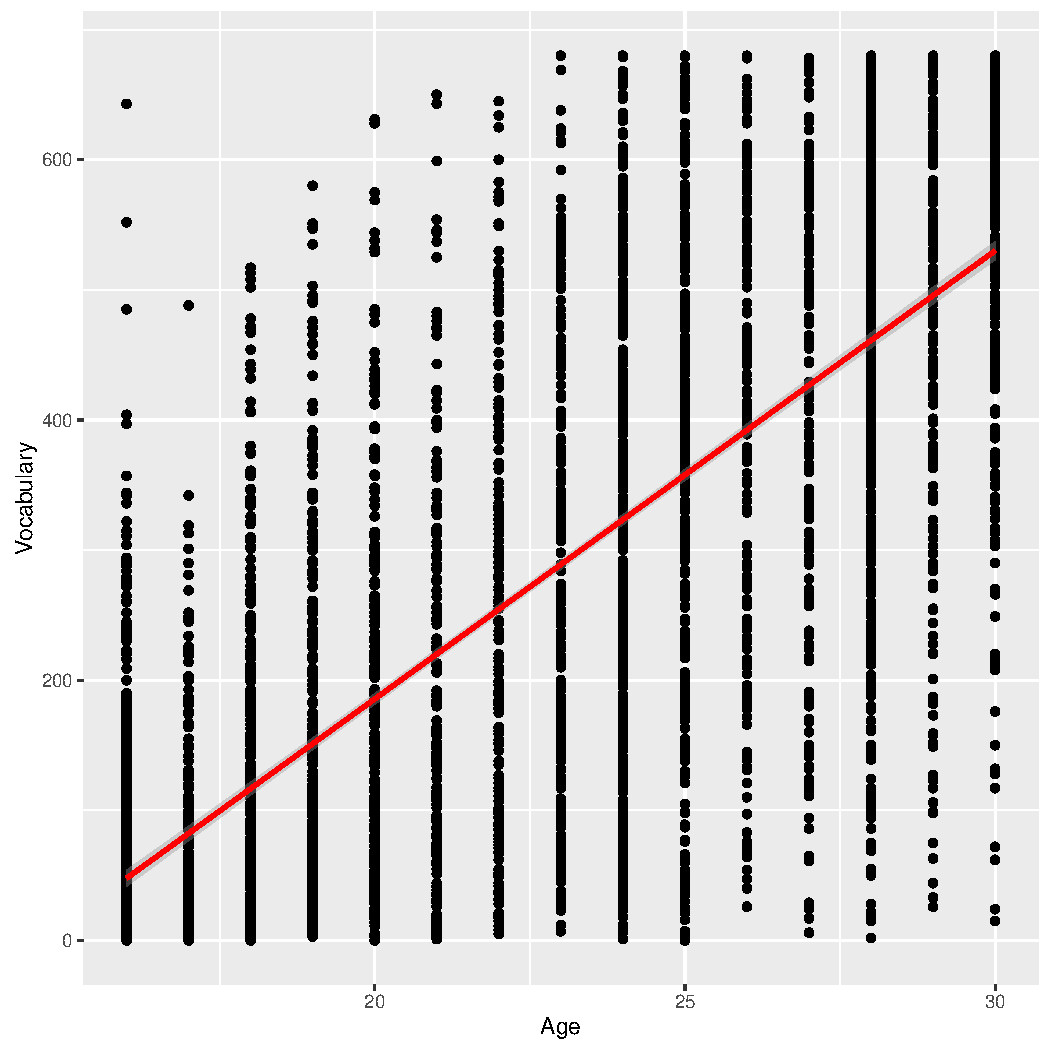
\includegraphics[width=\linewidth]{vocab_from_age.pdf}
        \caption{Vocab from Age}
        \label{fig:regression1}
      \end{figure}
      As the data shows, the average vocab is 1.793e+01 + 1.654-02 age. 
      \^{d} is the error, so 1.939e-04 can be multiplied with 0.96 to get the confidence
      interval. This means that we are 95\% confident that the actual slope, c, is
      within our interval. \newline Additionally, the line on the graph demonstrates the 
      projected slope, along with the fuzzy gray area showing our projected estimate
      for where the slope for the actual world may lie. Overall, one can clearly
      tell that as people get older, their vocabularies continue to go but slowly
      they learn at slower rates as people hit their late 20's. This is likely
      because most people finish college in their early-mid 20's and therefore
      are probably exposed to fewer new words after that. 
      

    \subsection*{Predict Vocab from Ethnicity}
      \begin{figure}[H]
        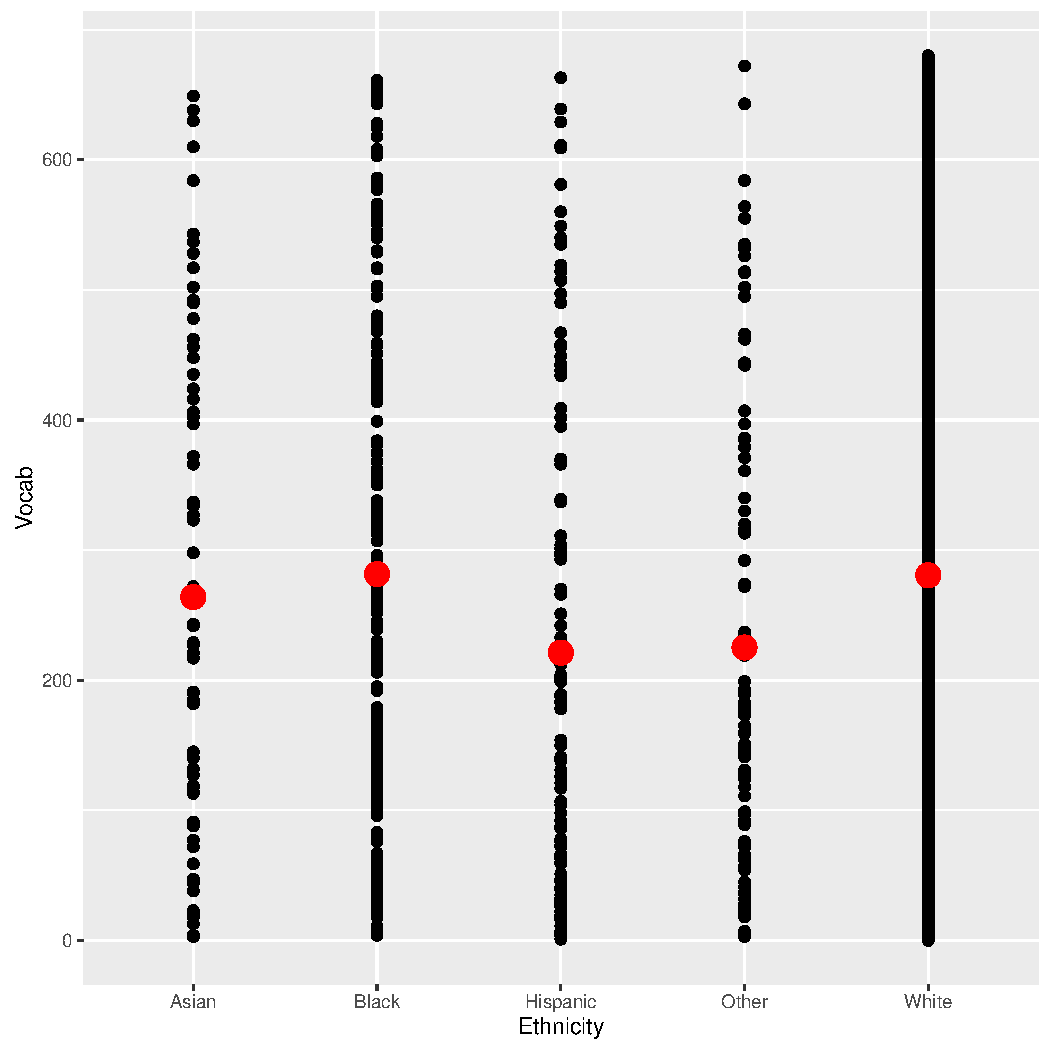
\includegraphics[width=\linewidth]{vocab_from_ethnicity.pdf}
        \caption{Vocab from Ethnicity}
        \label{fig:regression2}
      \end{figure}
      When I regressed Vocab with Ethnicity, I found that the average
      vocabulary size for Black is 263.94 + 17.63, 263.94 - 42.79 for Hispanic,
      263.94 - 38.79 for Other, and 263.94 + 16.73 for White. On the graph,
      these points are marked by the red circles. \newline
      In the data, there are 5 different ethnicities - Asian, Black, Hispanic, Other, 
      and White. In the results, Asian is omitted because the lm function automatically
      drops one term as the intercept. This data serves as a reference for all of the
      other data points. In other words, all of the other data points are measured
      relative to the intercept. In this case, 'Asian'. If this is avoided, and all
      of the different variables are included in linear regression, you get
      'perfect collinearity'. This happens when each variable only gets compared to itself.
      Regression without an intercept is often less accurate. 
      Also, to circumvent the problem of missing data, I used the omit option
      such that any line with a 'NA' value is automatically excluded and removed
      from calculations. 
      


    \subsection*{Predict Vocab from Mom's Education}
      \begin{figure}[H]
        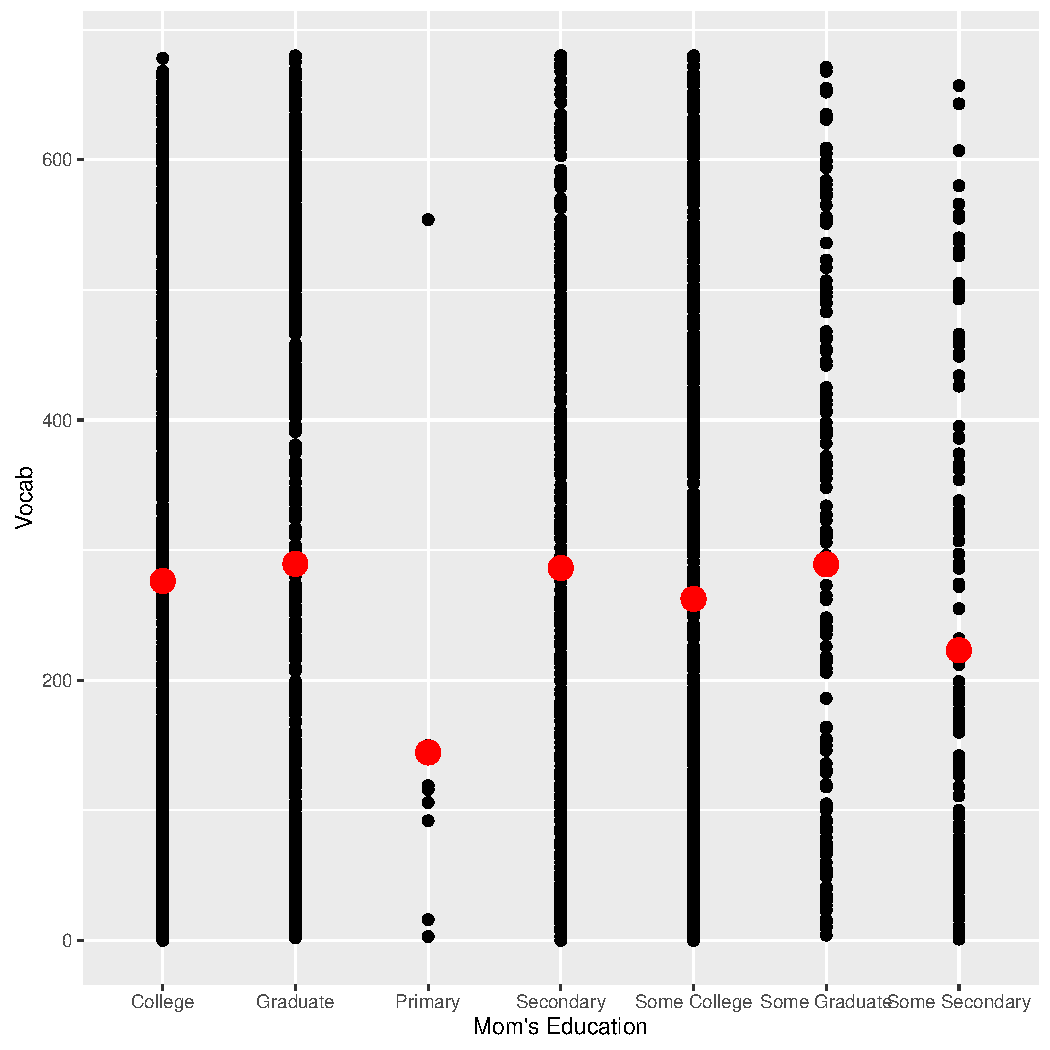
\includegraphics[width=\linewidth]{vocab_from_mom_ed.pdf}
        \caption{Vocab from Mom's Education}
        \label{fig:regression3}
      \end{figure}
      After a while, I realized that there were actually many combinations of data points
      that made logical sense for trends. The relationship between the Mother's education
      and the vocabulary of the child was the first to come to mind. In theory, given that one of the 
      parents has some degree of education, higher levels of education should imply
      larger vocabularies. 
      Through regression testing, I found that children whose parents completed
      Graduate school had vocab sizes of 276.229 + 13.148, Moms that only completed
      Primary school had children who knew drastically fewer words, 276.229 - 131.729,
      then children of mothers who completed some level of college had vocabularies of
      262.453, 288.312, and 223.047 for Some College, Some Graduate, and Some Secondary 
      respectively. 
      The last, Mothers with Some Secondary, is particularly significant because the p value
      is extremely small. This indicates that there is a significant relationship between
      the modeled regression and the actual data. 
      

    \subsection*{Predict Vocab from Age and Ethnicity}
      \begin{figure}[H]
        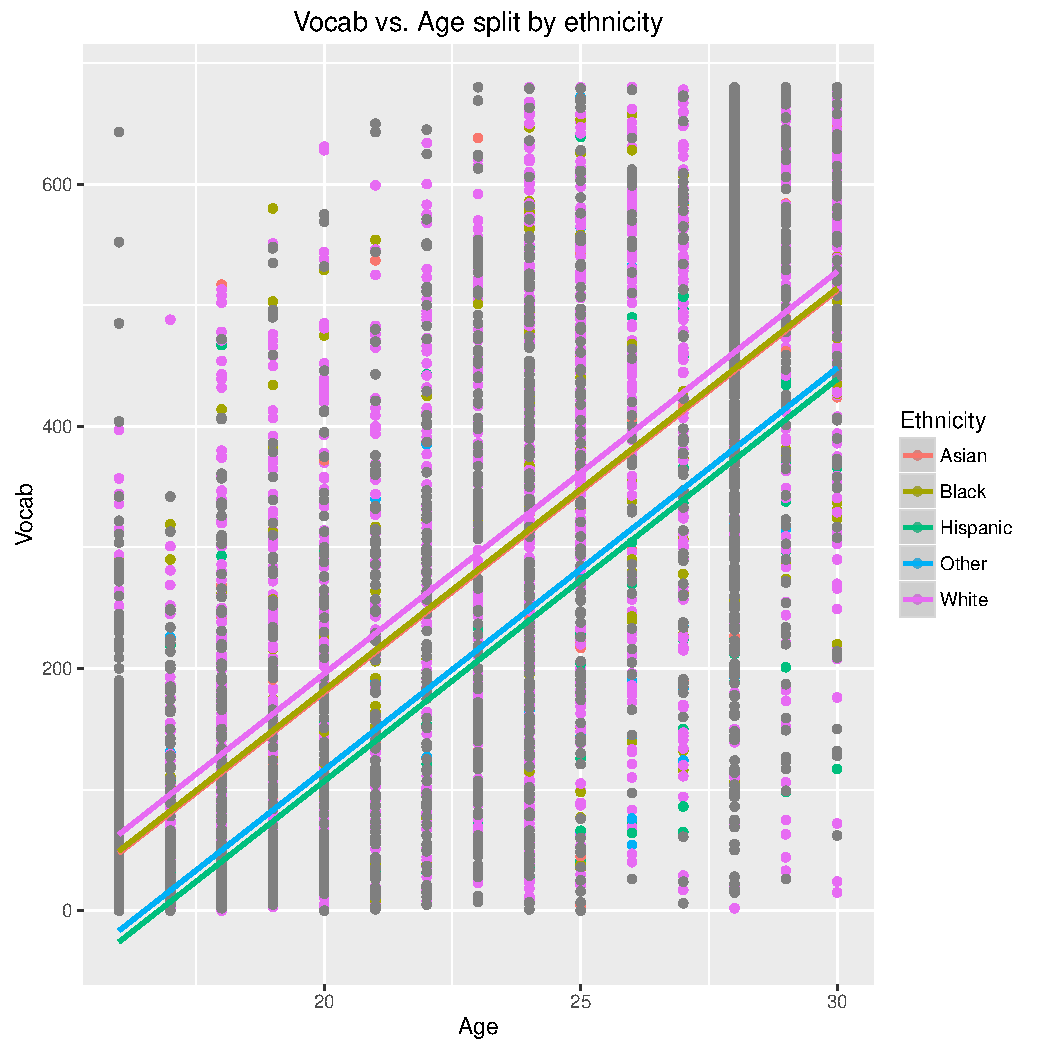
\includegraphics[width=\linewidth]{vocab_from_age_and_ethnicity.pdf}
        \caption{Vocab from age and ethnicity}
        \label{fig:regression3}
      \end{figure}
      In our first linear regression, we plotted and modeled vocabulary data solely from age, without any other filtration. Based on basic intuition on how vocabulary is developed, I determined that filtering this data based on ethnicity can yield some more results and ultimately insight into how individuals of different cultures have different vocabulary strengths. One way to do this is to regress age and vocabulary data and split models by ethnicity. \\
      Our regression results are particularly significant for some ethnicities and not so for others. Our regression results for Asian, Hispanic, and other ethnicities are extremely significant, with a significance p < 0.01 for all. This indicates that the data correlates very strongly; in other words these cultures do not cause much variance in the vocabulary strength of an individual. \\
      Conversely, our regression results for Black and White ethnicities have very high p-values, with 0.930101 and 0.383645, respectively. This indicates that Black and White households have extremely varying data when it comes to vocabulary strength of an individual from these households. This implies that such households have extremely distanced extremes for vocabulary strength.
      

\appendix
\section*{Code}
    \subsection*{A.R}
        \begin{lstlisting}[language=R]
# This function searches through all the needed files and gets rid of anything that has
# two vertical lines in a row. This allows R to read the files into a data frame properly.
convert <- function() {
  f = "ml-100k/u.item" #make a file object
  x <- readLines(f) #read in the file
  y <- gsub("\\|\\|", "\\|nodata\\| ", x) #search and replace || with |nodata|
  y <- gsub("'", "", y) #sub out quotes which mess up ordering
  cat(y, file=f, sep="\n") #Remake the file
}

#This function prepares the item file for the merging. It prepares 
# row and column titles, and separates them with commas for an output file
# for easy readability. This is done in a csv. 
itemf <- function () {
  convert()
  item <- read.table("ml-100k/u.item", sep="|", fill=TRUE) #read in item 
  names(item) <- c("MovieID", "title", "ReleaseDate", "vidreleasedate", "imdb", "Action", "Adventure", "Animation", "Children's", "Comedy", "Crime", "Documentary", "Drama", "Fantasy", "Film-Noir", "Horror", "Musical", "Mystery", "Romance", "Sci-Fi", "Thriller", "War", "Western") #assign new column titles
  write.table(item, file="item.csv", row.names=FALSE, col.names=TRUE, sep=",") #output the file in a csv.
  return(item)
}


#This function prepares the data file for the merging. It prepares 
# row and column titles, and separates them with commas for an output file
# for easy readability. This is done in a csv. 
dataf <- function() {
  data <- read.table("ml-100k/u.data", fill=TRUE) #read in user
  names(data) <- c("UserID", "MovieID", "Rating", "Timestamp")
  write.table(data, file="data.csv", row.names=FALSE, sep=",")
  return(data)
}

#This function prepares the user file for the merging. It prepares 
# row and column titles, and separates them with commas for an output file
# for easy readability. This is done in a csv. 
userf <- function() {
  user <- read.table("ml-100k/u.user", sep="|") #read in user
  names(user) <- c("UserID", "Age", "Gender", "Occupation", "ZIPCode")
  write.table(user, file="user.csv", row.names=FALSE, sep=",")
  return(user)
}

# this file merges the UserID and MovieID by data and user, then the merged with item.
# this creates a large file with all needed bits of information together.
mergef <- function () {
  d <- dataf()
  u <- userf()
  i <- itemf()
  two <- merge(d, u, by="UserID") #this works
  write.table(two, "two.csv", row.names=FALSE, col.names=TRUE, sep=",")# this works

  three <- merge(two, i, by="MovieID")
  write.table(three, "merged.csv", col.names=TRUE, row.names=FALSE, sep=",")
  return(three)
}

# this file removes unneeded fields, and gets names ready for problem A. 
# this method also removes duplicates for each user's ratings, and replaces them with the average
# this makes it so that each user only gets to 'vote' once.
splitf <- function() {
  merged <- mergef()
  cp <- userf()
  cp$Occupation <- NULL
  cp$ZIPCode <- NULL
  cp$Age<-NULL
  #break up into groups = by person
  #within each group, apply a function
  ready <- aggregate(merged$Rating, list(merged$UserID), mean, simple=FALSE) #original
  names(ready) <- c("UserID", "AverageRating")

  #merge
  ready <- merge(ready, cp, by="UserID")
  #delete columns until only id and gender, then merge that to ready.
  #end merge

  write.table(ready, "ready.csv", row.names=FALSE, col.names=TRUE, sep=",")
  return(ready)
}

# this method gets the tables ready for h. This is important because
# some fields have missing information and have to be removed. Also, 
# this allows the group to have different breakups depending on what
# field we want to be separated.
preph <- function() {
  merged <- mergef()
  cp <- userf()
  cp$Occupation <- NULL
  cp$ZIPCode <- NULL
  #break up into groups = by person
  #within each group, apply a function
  ready <- aggregate(merged$Rating, list(merged$UserID), mean, simple=FALSE) #original
  names(ready) <- c("UserID", "AverageRating")

  #merge
  ready <- merge(ready, cp, by="UserID")
  #delete columns until only id and gender, then merge that to ready.
  #end merge

  write.table(ready, "h.csv", row.names=FALSE, col.names=TRUE, sep=",")
  return(ready)
}

prepa <- function() {
  table <- mergeall()
  write.table(table, file="output.csv", sep=",")
}

aa <- function() { #problem 1 done
  #find an approximate 95% confidence intervalfor the population mean rating by men
    #find all men's ratings
    #find confidence interval
  #references: http://www.cyclismo.org/tutorial/R/confidence.html
  table <- splitf()
  #get all ratings from table where gender = M
  mtable <- subset(table, !(Gender %in% c("F"))) #grab data where v2 doesn't have F
  sdev <- sd(mtable$AverageRating)
  size <- nrow(mtable)
  mean <- sum(mtable$AverageRating)/size

  error <- qt(0.975, df=size-1) * sdev/sqrt(size)
  cat("95% interval:", mean-error, mean+error, "\n")
}

ab <- function() { #problem 2 done
  #find an approximate 95% confidence intervalfor the population mean rating by men
    #find all women's ratings
    #find confidence interval
  table <- splitf()
  #get all ratings from table where gender = F
  ftable <- subset(table, !(Gender %in% c("M"))) #grab data where v2 doesn't have F
  sdev <- sd(ftable$AverageRating)
  size <- nrow(ftable)
  mean <- sum(ftable$AverageRating)/size

  error <- qt(0.975, df=size-1) * sdev/sqrt(size)
  cat("95% interval:", mean-error, mean+error, "\n")
}

ac <- function() {
  #find approximate 95% interval for difference between two means
  table <- splitf()
  mindex <- table$Gender == "M"
  male <- table[mindex,]$AverageRating

  female <- table[!mindex,]$AverageRating
  print(t.test(male, female, var.equal = TRUE))
}

ad <- function() {#done
  table <- splitf()
  mtable <- subset(table, !(Gender %in% c("F")))
  ftable <- subset(table, !(Gender %in% c("M")))
  msize <- nrow(mtable)
  fsize <- nrow(ftable)
  xbar <- sum(mtable$AverageRating)/msize
  ybar <- sum(ftable$AverageRating)/fsize
  msdev <- sd(mtable$AverageRating)
  fsdev <- sd(ftable$AverageRating)
  se <- sqrt(msdev*msdev/msize + fsdev*fsdev/fsize)
  z = (xbar - ybar - 0)/se
  cat("Z: ", z, "\n", "For values of Z > 1.96, we reject the Hypothesis that the population means are equal\n")
}

ae <- function() { #done
  #plot male and female ratings on a histogram
  table <- splitf()
  ftable <- subset(table, !(Gender %in% c("M"))) #grab data where v2 doesn't have F
  mtable <- subset(table, !(Gender %in% c("F"))) #grab data where v2 doesn't have F

  library(ggplot2) #the plot object is the total sets of information needed
  #for ggplot. This allows us to save to a file, in savePlot. 
  # The first part sets the table, which is also the data used to graph.
  # the next line sets the first histogram - Male, and makes binwidth = 0.1.
  # This makes what is seemingly continous points into ranges, so that they can be
  # graphed on a histogram. The same is done on the last line, but for women.
  plot <- ggplot(table, aes(x=AverageRating))+
    geom_histogram(data = subset(table, Gender %in% c("M")), binwidth=0.1, fill="blue", alpha=0.2)+
    geom_histogram(data = subset(table, Gender %in% c("F")), binwidth=0.1, fill="red", alpha=0.2)

  savePlot(plot, "histogram.png")
}

savePlot <- function(plot, filename) {
  pdf(filename)
  print(plot)
  dev.off()
}

af <- function() {
  table <- splitf()
  n <- nrow(table)
  # calculate difference in sums of male and female raters
  k <- sum(table$Gender == "M") - sum(table$Gender == "F")
  pbar <- k / n     # calculate sample mean
  se <- sqrt(pbar * (1 - pbar) / n)   # calculate standard error
  e <- qnorm(0.975) * se
  print(pbar + c(-e, e))
}

ag1 <- function() { 
  table <- splitf()
  n <- nrow(table)
  k <- sum(table$Gender == "M")
  pbar <- k/n
  se <- sqrt(pbar * (1-pbar) / n)
  e <- qnorm(0.975) * se
  print(pbar + c(-e, e))
}

ag <- function() { 
  table <- splitf()

  n <- nrow(table)
  k <- sum(table$Gender == "M") #number of males
  print(prop.test(k, n))
  # find the number of males, and project the actual number in the real world
  # based off of the sample.
}

ah1 <- function() {
  table <- preph() 
  gender <- table$Gender #isolate the needed variables
  age <- table$Age
  gender <- as.integer(gender=="F") #make indicator varialbes by Gender
  y <- table$AverageRating
  fit <- lm(y ~ age + gender)
  print(summary(fit)) #figure out the needed information from linear regression from guessing from age and gender
  summaryfit <- summary(fit)
  fitcov <- vcov(fit) #fit the covariance
  se <- sqrt(fitcov[2,2])
  bAge <- coef(fit)[2]
  cat("95% Confidence interval for age coefficient: (", bAge-1.96*se,", ", bAge+1.96*se, ")\n")
  #make a function for a Z test
  cat("bAge = ", bAge, "\n")
  Z <- (bAge - 0)/se
  cat("Z = ", Z, "\n")

  if (Z > 1.96) cat("We reject The Hypothesis at the 5% level\n")
  if (Z > 1.96) cat("The p-value was ", (1 - pnorm(Z)) * 2, "\n")
}

ah2 <- function() {#done
  table <- preph()
  gender <- table$Gender
  age <- table$Age
  gender <- as.integer(gender=="F")
  
  y <- table$AverageRating
  fit <- lm(y ~ age + gender)
  h2val <- rbind(1, 28, 1)
  h2mean <- sum(coef(fit)*h2val)
  
  A <- vcov(fit)
  se <- sqrt( c(1,28,1) %*% A %*% h2val)
  cat("95% Confidence Interval for mean population rating among women of age 28: (", h2mean-(1.96*se),", ", h2mean+(1.96*se),")\n")
}

        \end{lstlisting}
        
    \subsection*{B.R}
        \begin{lstlisting}[language=R]
#TODO:
#Predict vocab size 
#From age
#From birth order
#Ethnicity
#Sex
#Mom's education

#univariate analysis - one variable




# This function reads in the table with needed information
prep <- function() {
  table <- read.table("vocabulary_norms_data.csv", sep=",", fill=TRUE, header=TRUE)
}

# This predicts vocab from the person's age, and graphs it
vocab_from_age <- function() {
  table <- prep()
  model <- lm(table$age~table$vocab) #predict vocab given age, and find correlation
  print(summary(model))

  # plot the given vocab for each age, and the trendline.
  # The plot object is for saving the image
  # the first line sets points as well as the data needed for creating the graph
  # The second line creates a line that goes through, to demonstrate trend.
  # The second and third line put in tites for what each label should be on the graph
  library(ggplot2)
  plot <- ggplot(model, aes(x=table$age, y=table$vocab)) + geom_point() + 
    stat_smooth(method="lm", col="red") + ylab(label = "Vocabulary") + 
      xlab("Age")

  savePlot(plot, "vocab_from_age.pdf")
}

# This is a function I created to save images
savePlot <- function(plot, filename) {
  pdf(filename)
  print(plot)
  dev.off()
}

# This will predict ethnicity from vocab
vocab_from_ethnicity <- function() {
  table <- prep()
  table <- na.omit(table) #get rid of the useless/unusable data
  model <- lm(table$vocab ~ table$ethnicity, data=table) #guess vocab from ethnicity
  #R makes indicator variables, so each ethnicity is separated and labeled
  print(summary(model)) #find the correlations between ethnicity and the amount
  # of vocab each person knows

  data1 <- data.frame(table$ethnicity, table$vocab) #Isolate the needed data
  library(ggplot2) #import ggplot 
  # The plot object is for outputting to a file
  # the first line lets use decide which function to plot the points on. It tries
  # to predict vocab given ethnicity. 
  # Each ethnicity is separated, and the average from vocab is added in
  plot <- ggplot(data1, aes(x=table$ethnicity, y=table$vocab)) +  
    geom_point(size=2) + 
      stat_smooth(method=lm) + ylab("Vocab") + xlab("Ethnicity") + 
        stat_summary(fun.y="mean", geom="point", color='red', size=5)
  savePlot(plot, "vocab_from_ethnicity.pdf")
}

vocab_from_mom_ed <- function() {
  table <- prep()
  table <- na.omit(table)
  model <- lm(table$vocab ~ table$mom_ed, data=table)
  print(summary(model))

  data1 <- data.frame(table$sex, table$vocab)
  library(ggplot2)
  plot <- ggplot(data1, aes(x=table$mom_ed, y=table$vocab)) + 
    geom_point(size=2) + 
      geom_smooth(method=lm) + ylab("Vocab") + xlab("Mom's Education") + 
        stat_summary(fun.y="mean", geom="point", color='red', size=5)
  savePlot(plot, "vocab_from_mom_ed.pdf")
}

vocab_from_age_and_ethnicity <- function() {
  table <- prep()
  model <- lm(table$vocab ~ table$age + table$ethnicity, data=table)
  print(summary(model))

  relevant <- table[c("vocab", "age", "ethnicity")]
  
  table$model <- stats::predict(model, newdata = table)
  err <- stats::predict(model, newdata=table, se=TRUE)
  table$ucl <- err$fit + 1.96 * err$se.fit
  table$lcl <- err$fit - 1.96 * err$se.fit
  
  Ethnicity <- table$ethnicity

  library(ggplot2)
  g <- ggplot(table)
  g <- g + geom_point(aes(x=table$age, y=table$vocab, color=Ethnicity))
  g <- g + geom_smooth(aes(x=table$age, y=model, color=Ethnicity))
  g <- g + labs(x = "Age", y = "Vocab")
  g <- g + ggtitle("Vocab vs. Age split by ethnicity")
  g <- g + scale_fill_discrete(name="Ethnicity")  
  savePlot(g, "vocab_from_age_and_ethnicity.pdf")
}

# NOT COMPLETE (problem with regression) 
vocab_from_momed_and_ethnicity <- function() {
        table <- prep()

  # assigning codes
  educodes <- as.integer(table$mom_ed)  
# print(head(educodes))
# print(head(table$mom_ed))
  collegeCode <- as.integer(educodes==1 | educodes==2 | educodes==5 | educodes==6)
  primaryCode <- as.integer(educodes==3)
  secondaryCode <- as.integer(educodes==4 | educodes==8)
  naCode <- as.integer(educodes==8)
        

  model <- lm(table$vocab ~ table$ethnicity + collegeCode + primaryCode + secondaryCode + naCode, data=table)
        print(summary(model))

        relevant <- table[c("vocab", "mom_ed", "ethnicity")]

        #plot(relevant)
        #plot(model)
        table$model <- stats::predict(model, newdata = table)
        err <- stats::predict(model, newdata=table, se=TRUE)
        table$ucl <- err$fit + 1.96 * err$se.fit
        table$lcl <- err$fit - 1.96 * err$se.fit

        Ethnicity <- table$ethnicity

        library(ggplot2)
        g <- ggplot(table)
        g <- g + geom_point(aes(x=table$mom_ed, y=table$vocab, color=Ethnicity))
        g <- g + geom_smooth(aes(x=table$mom_ed, y=model, color=Ethnicity))
        g <- g + labs(x = "Mother's Education", y = "Vocab")
        g <- g + ggtitle("Vocab vs. Mother's Education split by ethnicity")
        g <- g + scale_fill_discrete(name="Ethnicity") 
        savePlot(g, "vocab_from_momed_and_ethnicity.pdf")
}

# prints the currently displayed graph to the
# file filename; suffix can be "pdf", "png" or "jpg"
pr2file <- function (filename)
{
  origdev <- dev.cur()
  parts <- strsplit(filename,".",fixed=TRUE)
  nparts <- length(parts[[1]])
  suff <- parts[[1]][nparts]
  if (suff == "pdf") {
    pdf(filename)
  }
  else if (suff == "png") {
    png(filename)
  }
  else jpeg(filename)
  devnum <- dev.cur()
  dev.set(origdev)
  dev.copy(which = devnum)
  dev.set(devnum)
  dev.off()
  dev.set(origdev)
}

        \end{lstlisting}

\section*{Code Explanation}
  \subsection*{Problem A}
    Before I could start on anything else, I had to focus on how to change the merged data
    set from previous homework into something that I could use - something where
    each person's ratings was replaced with the average, and each user was only allowed
    to review one time. In order to do this, I first read in all of the different
    data sets - u.item, u.data, and u.user. I set the read.table() function
    to add in fill values in case they were missing so that everything would align. 
    I also replaced \textbar \textbar with \textbar nodata \textbar to prevent improper
    reading, through gsub. Next, after I read in each table, I put on appropriate 
    column titles. This was done through using names (tablename) = c("Title1", "Title2", etc.)
    Next, I merged my data together. I chose to merge by UserID for the data and users
    first, then with items by MovieID. At this point, I reached the problem of changing
    users who rated multiple times' ratings with the average. 
    For this, I created the splitf() function. This takes the original user table, 
    and deletes the Occupation, ZIPCode, and Age columns since these aren't needed
    for most of the steps. Then, I used aggregate to create a data frame with the mean rating
    per UserID instead. This was done with the line 
    aggregate(merged\$Rating, list(merged\$UserID), mean, simple=FALSE). This was 
    difficult because I tried using tapply() and split(), but these didn't return
    data frames. As a result, I replaced the function with aggregate and transformed
    the defining perameter (User ID's) into a list before entering. 
  \subsection*{Part a}
    Now, with prep finished, I set out on problems 1 and 2. These were rather similar,
    since I merely had to flip the Male/Female argument after I got one. For the first problem, 
    I started with my set-up table, as created by splitf(). From this,
    I took a subset of the table - all rows where Gender == Female were removed.
    Then, I found teh standard deviation with sd(), the size of my set with nrow(),
    and the mean through taking the sum of average ratings, then dividing by the size. 
    I then calculated the error with qt(0.975, df=size-1) because 0.975 would give
    me a 5\% interval, with degrees of freedom as one less than the set size.
    I multiplied this with the sdev/sqrt(size), and returned the mean +- the error.
  \subsection*{Part b}
    For this, I flipped the Male/Female argument from Problem 1.
  \subsection*{Part c}
    For problem 3, I found the 95\% interval for the difference between two means
    through finding the male averages and the female averages, then running it through
    t.test for the confidence interval.
  \subsection*{Part e}
    I pulled the set-up table from splitf(). Then, I created two opposite tables - one with
    all males and the other with all females. I plotted these on a histogram using
    their AverageRatings, setting different colors for each on the same graph
    to make it easy for the reader to recognize overlap. 
    \newline As you can see, Males and Females gave generally the same average voting, but
    Females were slightly more inclined to rate between 4 and 5 while males often rated
  \section*{Problem B}
    Since all of Problem B revolved around performing univariate and multivariate linear regressions, code for each function was relatively re-used. In order to regress points against each other, we first created a linear regression object (model), modeled data, and plotted the points and regression lines using geom\_point() and geom\_smooth() respectively.


\section*{Contributions}
  \subsection*{Vincent Yang:}
  \begin{itemize}
    \item Wrote code to replace \textbar \textbar with \textbar notext\textbar to be usable with 
      gsub search and replace. 
    \item Used aggregate to create a new data frame where each User was represented only once, in 
      preparation for Problem Set A. 
    \item Solved A.a
    \item Solved A.b
    \item Solved A.c
    \item Solved A.d
    \item Solved A.e using the 
      \lstset{language=R}
      \begin{lstlisting}
      hist()
      \end{lstlisting}
    \item Solved A.h
    \item Calculated and coded results and analysis for predicting Vocab from Age
    \item Calculated and coded results and analysis for predicting Vocab from Ethnicity
    \item Calculated and coded results and analysis for predicting Vocab from Mom's Education
    \item Completed \LaTeX  analysis for predicting Vocab from Age, with pictures
    \item Completed \LaTeX  analysis for predicting Vocab from Ethnicity, with pictures
    \item Completed \LaTeX  analysis for predicting Vocab from Mom's Education, with pictures
    \item Added explanations for Problem A code
  \end{itemize}

  \subsection*{Corey Nettleblad:}
  \begin{itemize}
  \item Solved A.d
  \item Solved A.h.1
  \item Solved A.h.2
  \item Did \LaTeX  writeup for A.d and A.h
  
  \end{itemize}

  \subsection*{Andy Yang:}
  \begin{itemize}
    \item Wrote code for A.f
    \item Wrote \LaTeX  writeup for A.a
    \item Wrote \LaTeX  writeup for A.b
    \item Wrote \LaTeX  writeup for A.c
    \item Wrote \LaTeX  writeup for A.d
    \item Wrote \LaTeX  writeup for A.f
    \item Wrote \LaTeX  writeup for A.g
    \item Cleaned up, corrected grammar of general \LaTeX  writeup
    \item Performed multivariate regression on problem B (Vocab vs. Age vs. Ethnicity)
    \item Performed multivariate regression on problem B (Vocab vs. Mother's Education vs. Ethnicity)
    \item Completed \LaTeX  analysis for predicting Vocab from Age and Ethnicity
    \item Completed \LaTeX  analysis for predicting Vocab from Mother's Education and Ethnicity
    \item Wrapped up submission, compiled files into tar and submitted
    \item Wrote code explanation for Problem B Code
  \end{itemize}



\end{document}

